\section{High-Level Design}
\label{sec:highlevel}

The system will have three major components: the tracking block, the gameplay
block, and the glove block.

\begin{figure}
\centering
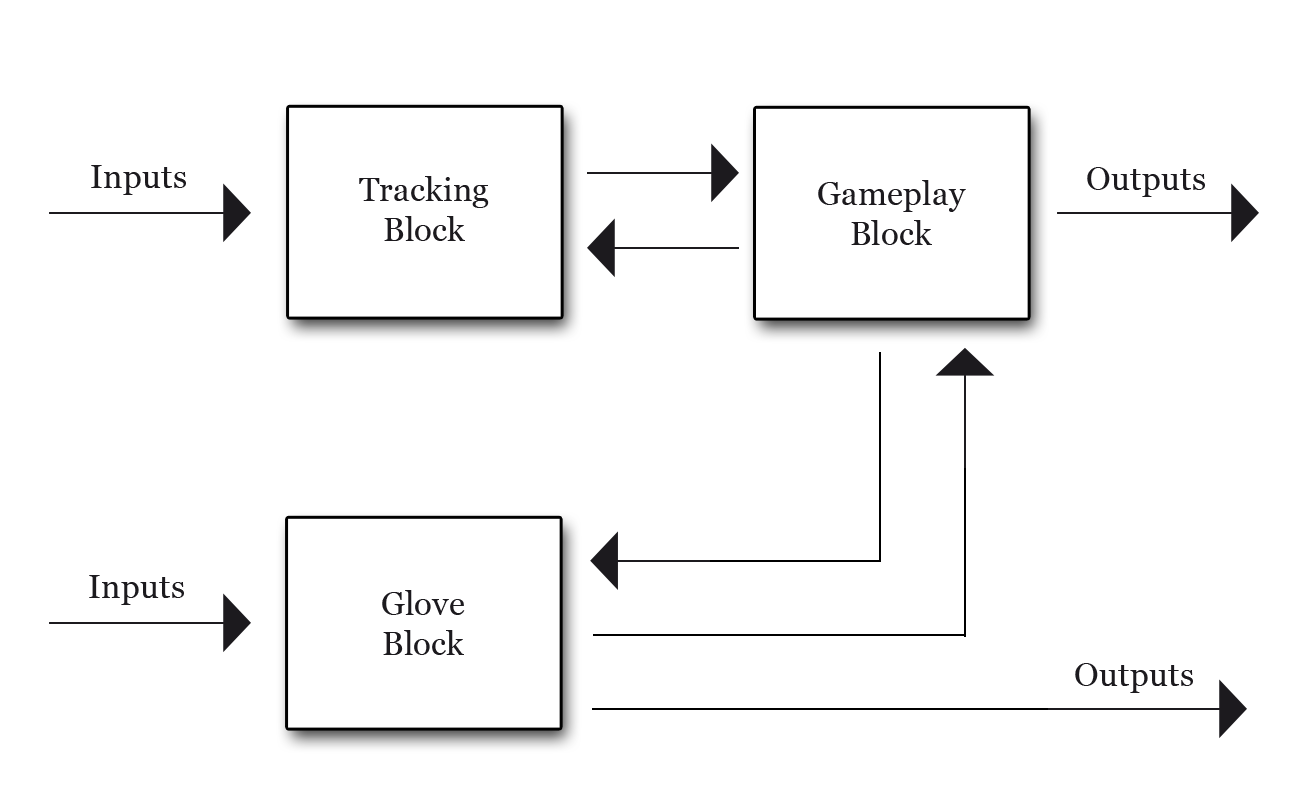
\includegraphics[scale=1]{img/high-level.png}
\caption{The high level block diagram shows the three major components of the
system: the tracking block, the glove block, and the gameplay block. It also
indicates information flow throughout the system}
\label{fig:high}
\end{figure}

\subsection{Tracking Block}

The Tracking block will take as input the frames and ancillary information from
the tracking camera. From this information it will determine the position of
each of the player's hands. That information will be output to the gameplay
block. This section will be constructed by Turner Bohlen.

\subsection{Gameplay Block}

The gameplay block will take as input the hand position from the camera block as
well as grab information from the glove block and control information from the
display. From this information, it will determine the location of the player on
the rock wall, the objects to display on screen, whether or not the user is
grabbing a handhold, and the pixel information to display in the next frame.
This section will be constructed by Chris Lang.

\subsection{Glove Block}

The glove block will manage inputs to and outputs from the gloves. It will take
information from the gameplay block describing if and how the user is touching
objects on screen and output feedback signals to the glove. It will also
debounce and output signals from the gloves' buttons. This section will be
constructed by Turner Bohlen.
